\documentclass[oneside,11pt]{amsart}

%\usepackage{a4wide}
%\usepackage{epsfig}
%\usepackage{psfig}
\usepackage{graphicx}
\usepackage{natbib,latexsym,url,enumitem,pdfpages}
\usepackage{color}
\usepackage{wrapfig}
\usepackage[belowskip=-10pt,aboveskip=0pt]{caption}
\usepackage{threeparttable}

\captionsetup{
    justification=justified,
    margin=0pt,
    font=small}

%%%%%%%%%%%%%%%%%%%%%%%%%%%%%%%%%%%%%%%%%%%%%%%%%%%%%%%%%%%%%%%%%%%%%%%%
% Allow for the okina; thanks to:
% https://tex.stackexchange.com/questions/424535/how-to-type-a-proper-hawai%CA%BBian-%CA%BBokina

\usepackage[utf8]{inputenc}
\usepackage{newunicodechar}
%\usepackage{libertine}

\DeclareRobustCommand{\okina}{%
  \raisebox{\dimexpr\fontcharht\font`A-\height}{%
    \scalebox{0.8}{`}%
  }%
}
\newunicodechar{ʻ}{\okina}
\newcommand{\hawaii}{Hawaiʻi}
%%%%%%%%%%%%%%%%%%%%%%%%%%%%%%%%%%%%%%%%%%%%%%%%%%%%%%%%%%%%%%%%%%%%%%%%

\newcommand{\arcsec}{\mbox{$^{\prime\prime}$}}
\newcommand{\gt}{$>$}

% Some fancy commenting
\definecolor{todo}{RGB}{200,0,0}
\newcommand{\comment}[2][todo]{{\color{#1}[[{\bf #2}]]}}

% Challenge counter
\newcounter{chalno}
\newcommand{\chal}[1]{\refstepcounter{chalno}\label{#1}}

% User commands
\makeatletter
\let\jnl@style=\rm
\def\ref@jnl#1{{\jnl@style#1}}

\def\ref@jnl#1{{\jnl@style#1}}% 
\newcommand\aj{\ref@jnl{AJ}}%        % Astronomical Journal 
\newcommand\araa{\ref@jnl{ARA\&A}}%  % Annual Review of Astron and Astrophys 
\newcommand\apj{\ref@jnl{ApJ}}%    % Astrophysical Journal ++
\newcommand\apjl{\ref@jnl{ApJL}}     % Astrophysical Journal, Letters 
\newcommand\apjs{\ref@jnl{ApJS}}%    % Astrophysical Journal, Supplement 
\newcommand\ao{\ref@jnl{ApOpt}}%   % Applied Optics ++
\newcommand\apss{\ref@jnl{Ap\&SS}}%  % Astrophysics and Space Science 
\newcommand\aap{\ref@jnl{A\&A}}%     % Astronomy and Astrophysics 
\newcommand\aapr{\ref@jnl{A\&A~Rv}}%  % Astronomy and Astrophysics Reviews 
\newcommand\aaps{\ref@jnl{A\&AS}}%    % Astronomy and Astrophysics, Supplement 
\newcommand\azh{\ref@jnl{AZh}}%       % Astronomicheskii Zhurnal 
\newcommand\baas{\ref@jnl{BAAS}}%     % Bulletin of the AAS 
\newcommand\icarus{\ref@jnl{Icarus}}% % Icarus
\newcommand\jrasc{\ref@jnl{JRASC}}%   % Journal of the RAS of Canada 
\newcommand\memras{\ref@jnl{MmRAS}}%  % Memoirs of the RAS 
\newcommand\mnras{\ref@jnl{MNRAS}}%   % Monthly Notices of the RAS 
\newcommand\pra{\ref@jnl{PhRvA}}% % Physical Review A: General Physics ++
\newcommand\prb{\ref@jnl{PhRvB}}% % Physical Review B: Solid State ++
\newcommand\prc{\ref@jnl{PhRvC}}% % Physical Review C ++
\newcommand\prd{\ref@jnl{PhRvD}}% % Physical Review D ++
\newcommand\pre{\ref@jnl{PhRvE}}% % Physical Review E ++
\newcommand\prl{\ref@jnl{PhRvL}}% % Physical Review Letters 
\newcommand\pasp{\ref@jnl{PASP}}%     % Publications of the ASP 
\newcommand\pasj{\ref@jnl{PASJ}}%     % Publications of the ASJ 
\newcommand\qjras{\ref@jnl{QJRAS}}%   % Quarterly Journal of the RAS 
\newcommand\skytel{\ref@jnl{S\&T}}%   % Sky and Telescope 
\newcommand\solphys{\ref@jnl{SoPh}}% % Solar Physics 
\newcommand\sovast{\ref@jnl{Soviet~Ast.}}% % Soviet Astronomy 
\newcommand\ssr{\ref@jnl{SSRv}}% % Space Science Reviews 
\newcommand\zap{\ref@jnl{ZA}}%       % Zeitschrift fuer Astrophysik 
\newcommand\nat{\ref@jnl{Nature}}%  % Nature 
\newcommand\iaucirc{\ref@jnl{IAUC}}% % IAU Cirulars 
\newcommand\aplett{\ref@jnl{Astrophys.~Lett.}}%  % Astrophysics Letters 
\newcommand\apspr{\ref@jnl{Astrophys.~Space~Phys.~Res.}}% % Astrophysics Space Physics Research 
\newcommand\bain{\ref@jnl{BAN}}% % Bulletin Astronomical Institute of the Netherlands 
\newcommand\fcp{\ref@jnl{FCPh}}%   % Fundamental Cosmic Physics 
\newcommand\gca{\ref@jnl{GeoCoA}}% % Geochimica Cosmochimica Acta 
\newcommand\grl{\ref@jnl{Geophys.~Res.~Lett.}}%  % Geophysics Research Letters 
\newcommand\jcp{\ref@jnl{JChPh}}%     % Journal of Chemical Physics 
\newcommand\jgr{\ref@jnl{J.~Geophys.~Res.}}%     % Journal of Geophysics Research 
\newcommand\jqsrt{\ref@jnl{JQSRT}}%   % Journal of Quantitiative Spectroscopy and Radiative Trasfer 
\newcommand\memsai{\ref@jnl{MmSAI}}% % Mem. Societa Astronomica Italiana 
\newcommand\nphysa{\ref@jnl{NuPhA}}%     % Nuclear Physics A 
\newcommand\physrep{\ref@jnl{PhR}}%       % Physics Reports 
\newcommand\physscr{\ref@jnl{PhyS}}%        % Physica Scripta 
\newcommand\planss{\ref@jnl{Planet.~Space~Sci.}}%  % Planetary Space Science 
\newcommand\procspie{\ref@jnl{Proc.~SPIE}}%      % Proceedings of the SPIE 

\newcommand\actaa{\ref@jnl{AcA}}%  % Acta Astronomica
\newcommand\caa{\ref@jnl{ChA\&A}}%  % Chinese Astronomy and Astrophysics
\newcommand\cjaa{\ref@jnl{ChJA\&A}}%  % Chinese Journal of Astronomy and Astrophysics
\newcommand\jcap{\ref@jnl{JCAP}}%  % Journal of Cosmology and Astroparticle Physics
\newcommand\na{\ref@jnl{NewA}}%  % New Astronomy
\newcommand\nar{\ref@jnl{NewAR}}%  % New Astronomy Review
\newcommand\pasa{\ref@jnl{PASA}}%  % Publications of the Astron. Soc. of Australia
\newcommand\rmxaa{\ref@jnl{RMxAA}}%  % Revista Mexicana de Astronomia y Astrofisica

%% added feb 9, 2016
\newcommand\maps{\ref@jnl{M\&PS}}% Meteoritics and Planetary Science
\newcommand\aas{\ref@jnl{AAS Meeting Abstracts}}% American Astronomical Society Meeting Abstracts
\newcommand\dps{\ref@jnl{AAS/DPS Meeting Abstracts}}% American Astronomical Society/Division for Planetary Sciences Meeting Abstracts



\let\astap=\aap 
\let\apjlett=\apjl 
\let\apjsupp=\apjs 
\let\applopt=\ao 



\DeclareRobustCommand{\gtrsim}{%
\mathrel{\hskip-.5em\begin{array}{c}>\\[-8pt]\sim\end{array}\hskip-.5em}}
\DeclareRobustCommand{\lesssim}{%
\mathrel{\hskip-.5em\begin{array}{c}<\\[-8pt]\sim\end{array}\hskip-.5em}}


\pretolerance=10000
\textwidth=6.4in
\textheight=8.95in
\voffset = 0.in
%\voffset = -0.3in  % For my printer
\topmargin=0.0in
\headheight=0.00in
\hoffset = 0.0in
%\hoffset = 0.33in  %  For my printer
\headsep=0.00in
\oddsidemargin=0in
\evensidemargin=0in
\parindent=2em
\parskip=0.2ex
 
\renewcommand{\baselinestretch}{1.03}

\special{papersize=8.5in,11in}

\newcommand{\markus}{\textcolor{green}}

\setlength{\parskip}{0.6 ex plus 0.4ex minus 0.2ex} \flushbottom
\pagestyle{plain} 

\begin{document}
% \thispagestyle{empty}

\pagenumbering{arabic}

\vspace*{-1.5cm}

\centerline{\textsf {\Large FOBOS: A Next-Generation Spectroscopic Facility}}
\centerline{\textsf {\large Response to Astro2020 Request for Information}}

\setcounter{page}{1}

\section*{Executive Summary}

% - Summarize your science objectives and your technical implementation at
%   a high level.

\noindent{\bf Science objectives:} FOBOS, the Fiber-Optic Broadband
Optical Spectrograph, is a facility-class, general-purpose
spectrograph for the 10m Keck II telescope. It emphasizes UV
sensitivity (up to the atmospheric limit), high multiplex, multiple
focal-plane sampling formats, and near Poissonian-level performance
over extremely long ($\sim$100 hr) integration times. These emphases
establish FOBOS's uniqueness among the suite of spectrographs coming
online for 8-10m class telescopes in the next decade. FOBOS is
specifically built to enable the deep spectroscopic follow-up of
upcoming large-scale imaging surveys (LSST, WFIRST, and Euclid)
identified as a significant need of the astronomy community in the US
and beyond. For example, capitalizing on the combined $\approx$\$4B
the US is investing in these imaging surveys, FOBOS can increase
LSST's dark-energy figure-of-merit by 40\% (Newman et al.\ 2015).

\smallskip

\noindent{\bf Technical implementation:} FOBOS is a fiber-fed,
fixed-format spectrograph. Its primary systems include (1) a
compensating lateral atmospheric dispersion corrector (CLADC), (2) a
robotic fiber-positioning system based on AAO's Starbug technology,
(3) micro-assembly fore-optics required to optimally couple the Keck
II input beam to the fiber feed, (4) 10m-long fiber trains that
provide at least three focal-plane sampling options (single fibers,
multiple small IFUs, and a single large-format IFU), and (5) a bank
of three 4-channel spectrographs that provide a simultanous spectral
range of 0.31-1 $\mu$m at a resolution of $R\sim3500$ across the full
band.

\smallskip

% - Summarize the technology maturity of your implementation, listing the
%   demonstrated technologies and the technologies requiring development.

\noindent{\bf Technological maturity:} FOBOS is nearing the end of
its conceptual design phase, and will begin its preliminary design
phase in Oct 2020, contingent on funding. Components of this document
represent significant improvements in FOBOS's design since the
completion of our Astro2020 submission. Although requiring
significant design work, FOBOS's backend systems are built on
well-established technologies: FOBOS's spectrographs and fiber train
inherit significantly from SDSS, MaNGA, and DESI designs. FOBOS's
front-end leverages the more than 15 years of development of the
Starbugs position system, which have been deployed and are in the
final commissioning stages for the TAIPAN instrument on the AAT.
Further development of the Starbugs technology is needed for use in
FOBOS; however this represents a 2nd-generation implementation of the
technology and will leverage simultaneous development of the
GMT/MANIFEST instrument. Further development of the micro-assembly
fore-optics is also necessary; prototypes are currently being
developed with potential industry partners and tested at UCO/UCB.

\smallskip

% - Summarize areas where the data to support this RFI are not currently
%   available.

\noindent{\bf Limitations of this RFI:} Given this early stage in
development, particular project components with limited extant
data/information to address this RFI are as follows:

\newpage

\section{Science}

% - Briefly describe the scientific objectives and the most important
%   measurements required to fulfill these objectives. Feel free to refer
%   to science white papers or references from the literature.

FOBOS, the Fiber-Optic Broadband Optical Spectrograph, is a
facility-class, general-purpose spectrograph for the 10m Keck II
telescope. Although its scientific use is expected to be very broad,
FOBOS meets an explicit need of the astronomy community in the era of
deep imaging surveys, like LSST, WFIRST, and Euclid, allowing for
highly efficient follow-up spectroscopy of faint sources using one of
the world's largest telescope. The design of the instrument reflects
this need by emphasizing high target densities, multiple focal-plane
sampling formats, blue sensitivity, and a stabilized and
well-calibrated instrument performance. To help establish these
requirements, we have outlined three ``design-reference'' key science
programs that facilitate the definition of FOBOS's instrument
requirements. These key programs are:

\smallskip

\noindent{\bf (a) Dark Energy}: Distance measurements for the
billions of sources in deep-imaging campaigns, like LSST, WFIRST, and
Euclid, will hinge on the use of photometric redshifts (photo-$z$s).
FOBOS observations that target $\sim$15k sources with $24 > i_{\rm
AB} > 25.3$ in specific regions of galaxy color space (cf.\
\comment{Masters et al.}) can dramatically improve the photo-$z$
accuracy applied to the full LSST sample, equivalent to an {\em
increase of LSST's dark energy figure-of-merit by 40\%} (Newman et
al.\ \comment{refs}). The {\it key instrument requirements} derived
from this program are (1) the blue wavelength coverage (down to the
atmospheric limit) to eliminate the usual "redshift desert", (2)
long-term stability of the instrument to allow for
near-Poisson-limited data reduction for ultra-deep, $\sim$100-hr
integrations, and (3) high multiplex to meet the target-density needs
of sources to $i_{\rm AB} > 25.3$ ($\sim$40 per arcmin$^2$).

\smallskip

\noindent{\bf (b) The baryonic ecosystem of galaxies at cosmic high
noon}: Mapping the crucial link between galaxies at $z\sim$2--3 and
the extended gas reservoirs, diffuse halos, and streaming filaments
that dominate the mass and regulate galaxy evolution in these
environments requires an instrument like FOBOS, even in the era of
JWST and ELTs. Its deep sensitivity and high sampling density enables
comprehensive tomographic reconstruction of the intergalactic medium
(IGM) across the largest cosmic structures in a single pointing
($\sim$10 transverse Mpc at $z \sim 2.5$). Its blue sensitivity
probes Ly-$\alpha$ across the complete formation epoch ($z =
1.5$--3.5) and opens access to high-ionization transitions that
reveal diffuse gas \emph{in emission}, such as O VI (1032 \AA).
Finally, its ability to combine single-fiber and multiplexed IFU
observations allows us to map the density and dynamical state of
diffuse gas at all relevant scales from the IGM to the circumgalactic
medium (CGM). The {\it key instrument requirements} derived from this
program parallel those from our ``Cosmology'' program, and
additionally require an integral-field mode that provides
two-dimensional kinematic data.

\smallskip

\noindent{\bf (c) The chemodynamical history of M31}: Compared to
existing and forthcoming spectrographs (e.g., PFS, MSE), FOBOS's high
sampling density and IFU modes offer unique capabilities for
efficiently mapping the high-source-density M31 disk. Building on
previous imaging (PHAT; \comment{ref}) and spectroscopy (SPLASH;
\comment{ref}) FOBOS will provide high-S/N spectra of $\sim$100k M31
disk stars that connect [Fe/H] and [$\alpha$/Fe] patterns to the
underlying dynamics. FOBOS will use integral-field observations of
$\sim$150 young stellar clusters that yield their present-day mass
function. Additionally, a few larg-scale star-formation complexes are
observed with FOBOS's monolithic IFU (FOV $\sim$ 700 arcmin$^2$)
allow for comparison of the local star-formation activity with the
Milky Way. In general, integral-field observations of the M31 disk
enable unique background-subtraction techniques that more accurately
remove the underlying diffuse M31 light, unavailable to single-fiber
observations. Combining these FOBOS observations with integral-field
data from the SDSS-V Local Volume Mapper and PFS/MSE surveys of halo
structure, a complete picture of the Andromeda system's formation
history will address key questions about disk evolution, dwarf
galaxies, and dark matter substructure with a level of statistical
power that has so far been limited to the Milky Way. The {\it key
instrument requirements} derived from this program parallel our
previous programs and additionally motivate the monolithic
integral-field unit.

Beyond the scope and requirements of these ``design reference''
programs, {\bf FOBOS enables a broad range of observations}, e.g.:
Milky Way and M31 halo stars and substructure; the Milky Way bulge;
globular clusters; variable stars from cadenced LSST imaging; dwarf
galaxies; rapid time-domain followup with an always-ready IFU;
structure of Coma and Virgo galaxies with IFUs and using globular
clusters and PNe as tracers; large IFU samples at $z \sim 1$ of 2D
emission-line kinematics; galactic winds; radial stellar-population
trends from stacked spectra at $z \sim 1$; environmental group
identification at $z \sim 1$--2; galaxy cluster and proto-cluster
followup; QSO light echos in the IGM; and redshift calibration of LBG
samples at $z = 1.5$--5 for CMB lensing cross-correlation.

Finally, given the wealth of photometric data and the continued
increase in sophistication and broad application of state-of-the-art
machine-learning techniques, we expect a common theme of FOBOS
observations to be the build-up of optimized training samples. We
have already seen the power of the combination of large samples of
photometric or low-spectral-resolution data with higher resolution
training sets in inferring higher-order properties. Examples include
stellar parameters (age, metallicity, $\log g$, $T_{\rm eff}$) and
distance (e.g., Ting et al. 2018a,b) and emission-line fluxes in
galaxy spectra (e.g., Capak).

% - Of the objectives, which are the most demanding? Why?
% - Present the highest-level technical requirements (e.g. spatial and
%   spectral resolution, sensitivity, timing accuracy) and their relation
%   to the science objectives.

\subsection{Top-level Requirements}

FOBOS's current top-level requirements are provided in Table
\ref{tab:reqs}; however, we caution that these are still under
development.

Deep exposures.  Keeping near Poissonian performance for 100 hours.


% - For each performance requirement identified, describe as
%   quantitatively as possible the sensitivity of the science objectives
%   to achieve the requirement.  If you fail to meet a key requirement,
%   what would be the impact on achieving the science objectives?


\begin{table}[h!]
\centering
\begin{threeparttable}
\caption{FOBOS Top-Level Requirements}
\footnotesize
\begin{tabular}{| l | c | p{2.5cm} | p{1.5cm} | p{4cm} |}
\hline
{\bf Description} & {\bf ID} & {\bf Requirement} & {\bf Goal} & {\bf Justification} \\
\hline
\hline
Field of View & TOP.REQ.A01 & $D=17^{\prime}$ & $D=20^{\prime}$ & Maximum FoV matches full Keck-Nasmyth FoV \\
\hline
Single-fiber multiplex & TOP.REQ.A02 & 1800 &  & Achieve density of 6 arcmin$^2$ for $20^{\prime}$ FoV \\
\hline
Single-fiber aperture & TOP.REQ.A03 & $0.7^{\prime} < D < 1.3^{\prime}$ &  & Optimize S/N of extracted spectra given WMKO seeing distribution \\
\hline
Calibration bundles & TOP.REQ.A10 & 12 7-fiber bundles & & Flux calibration fidelity; four per spectrograph (Yan et al. 2016) \\
\hline
mini-IFU size & TOP.REQ.A04 & $\gtrsim$5\arcsec &  & Cover scales of $\gtrsim$20 kpc at $z=2-2.5$ \\
\hline
mini-IFU sampling & TOP.REQ.A05 & $\lesssim$0.8\arcsec & & Optimize extended-source spectroscopy \\
\hline
mini-IFU multiplex & TOP.REQ.A06 & 45 & & 37 fibers per IFU, 15 IFUs per spectrograph \\
\hline
Wavelength coverage & TOP.REQ.A07 & 0.31 - 1 $\mu$m & & Eliminate redshift desert \\
\hline
Spectral Resolution & TOP.REQ.A08 & $R = 3500$ & & Subtraction of night-sky lines in the red \\
\hline
Throughput & TOP.REQ.A09 & $\gtrsim$30\% over 95\% of the bandpass & & Competitive with other upcoming instruments \\
\hline
\end{tabular}
\begin{tablenotes}
\item Mini-IFU requirements above are optimized for the CGM science case; however, we expect additional IFU modes to be explored, including those that subsample the median Keck seeing (0.3 arcsec) and those that take advantage of a GLAO mode should one be available at Keck.
\end{tablenotes} 
\label{tab:reqs}
\end{threeparttable}
\end{table}

\section{Enabling Technology}
\label{sec:tech}

% - Please provide information describing new enabling technologies
%   required for activity success.

There are no fundamentally new technologies needed to enable the
FOBOS concept to move ahead. However, there are a few key
technologies that either require modifications and development of
existing designs for there specific use in FOBOS.

FOBOS's conceptual design includes fused-silica etched (FSE) gratings
in each channel of our 4-channel spectrographs. To date, FSE gratings
have had limited use in astronomical instruments; however, FSE
grating advancement has come quickly on the heels of development of
e-beam lithography techniques, which allow shaping of grating grooves
to nanometer precision. Custom designed gratings promise high
efficiency over our entire wavelength range. In particular, their use
in FOBOS overcomes a lack of volume-phase holographic (VPH) gratings
with good transmission at wavelengths shorter than 350 nm.
Prototyping and testing of these diffractive optics will be ongoing
during our preliminary design phase. If necessary, our design can be
rescoped to use VPH gratings with appropriate compensations to the
rest of the design given their limitations.

Additional key design elements are:
%
\begin{enumerate}
\item Implementation of a compensating lateral atmospheric dispersion
corrector (CLADC) that includes a fold mirror between its 2nd and 3rd
elements. The mirror folds the incoming beam such that the face of
the final element of the CLADC is perpendicular to the gravity vector
and serves as the drive surface for the Starbugs positioning system
(see below). This orientation dramatically decreases the risk of
Starbug adhesion failures on the drive surface.
\item Development and process testing of micro-assembly foreoptics
composed of single lenses for single-fiber apertures and micro-lens
arrays for integral-field apertures.
\item Integration of both single-aperture and multi-aperture arrays
assemblies in the Starbugs piezo assembly.
\item Roughly an order-of-magnitude increase in the number of Starbugs
simultaneously used in a positioning system.
\end{enumerate}

% - Please indicate any non-US technology required for activity success
%   and what back up plans would be required if only US participation
%   occurred. 

\subsection{Non-US Technologies}
\label{sec:starbugs}

The FOBOS robotic focal-plane positioning system uses the Starbugs
technology, developed exclusively by Australian Astronomical Optics
at Macquarie University in Sydney, Australia. No similar technology
exists from a US vendor or otherwise. The Starbugs technology is very
attractive for FOBOS for three reasons: (1) It has the potential to
allow for multiple focal-plane modules specifically designed with an
exchange procedure that can be performed during daytime telescope
operations. (2) Similarly, the system allows for upgrade paths that
add new focal-plane sampling modes/modules that either interface with
the currently proposed FOBOS spectrographs or new spectrographs that
provide expanded capabilities (e.g., higher spectral resolution). (3)
Starbugs allow for the very large patrol radii needed for the
mini-IFU modes, in particular.

Starbugs are currently deployed by the TAIPAN instrument on the
Anglo-Australian Telescope (AAT). TAIPAN's commissioning phase has
proven critical to the refinement of the Starbugs design, and the
instrument is nearly ready to enter normal operations. AAO is deeply
invested in the future of the Starbugs technology, both via our
interest in their use in FOBOS, but also via their development of
MANIFEST, a front-end for the first-light spectrographs built for the
Giant Magellan Telescope.

In the event that the Starbugs technology becomes untenable for
implementation in FOBOS, we will explore zonal position systems
similar to those used by DESI, PFS, and SDSS-V. This may require a
descope of the number of focal-plane sampling modes available or
exploration of other technologies that may enable these modes, such
as highly efficient fiber switching.

% - For any technologies that have not been demonstrated by sub-scale or
%   full-scale models as of this request, please describe the rationale
%   for your technical maturity assessment, including the description of
%   analysis or hardware development activities to date, and its
%   associated technology maturation plan.
% TODO: Come back to this.

% - Describe the aspect of the enabling technology that is critical to the
%   concept’s success, and the sensitivity of mission performance if the
%   technology is not realized or is only partially realized.
% TODO: Assess the sensitivity of FOBOS to each of the technologies listed above?

% - Provide cost and schedule assumptions by year for all development
%   activities, and the efforts that allow the technology to be ready when
%   required, as well as an outline of readiness tests to confirm
%   technical readiness level.
% TODO: Just refer to the cost section?

\section{Telescope}

FOBOS is an instrument planned for the existing Keck II telescope.
Installation, integration, and commissioning of the instrument are
minimally described in our work breakdown structure (see Section
\ref{sec:cost}), with specific details to be worked out in
consultation with our Keck partners during our upcoming preliminary
design phase.
 
% These details are irrelevant to FOBOS:
% - Provide an overview description of the characteristics and
%   requirements of the optical telescope(s), antenna(s), or collector(s)
%   highlighting key capabilities and any residual technology risks. 
% - Provide diagrams or drawings showing the observatory or antenna array
%   with the instruments and other components labeled and a descriptive
%   caption.
% - Please provide any available review packages (e.g. Conceptual Design
%   Review, Preliminary Design Review) that describe the scope of
%   technical design and implementation.
% - Please describe any hardware/software with significant heritage.
% - Please fill out the table below regarding the primary scientific
%   equipment (e.g., Telescope or Antenna Array). Expand, contract, or
%   modify this table as necessary and applicable.
% - Identify and describe the three components of lowest technical
%   maturity, and explain how and when these components will be
%   demonstrated in hardware.
% - What are the three greatest risks to cost, schedule, and performance?
% - Describe any aspect of the design or implementation that may require
%   non-US participation.

\section{Instrumentation}

% - Describe the proposed science instrumentation, and briefly state the
%   rationale for selection. Discuss the capabilities of each instrument
%   (Inst #1, Inst #2 etc.) and how the instruments are used together.
%   Indicate whether cryogens or other cooling are required. 

% - Briefly describe any concept, feasibility, or definition studies
%   already performed and please provide any available Review Packages
%   (e.g., Conceptual Design Review, Preliminary Design Review) that
%   describe the instrument and its design and implementation.

\subsection{Conceptual Design}

\begin{figure}[h!]
\vskip -0.1in
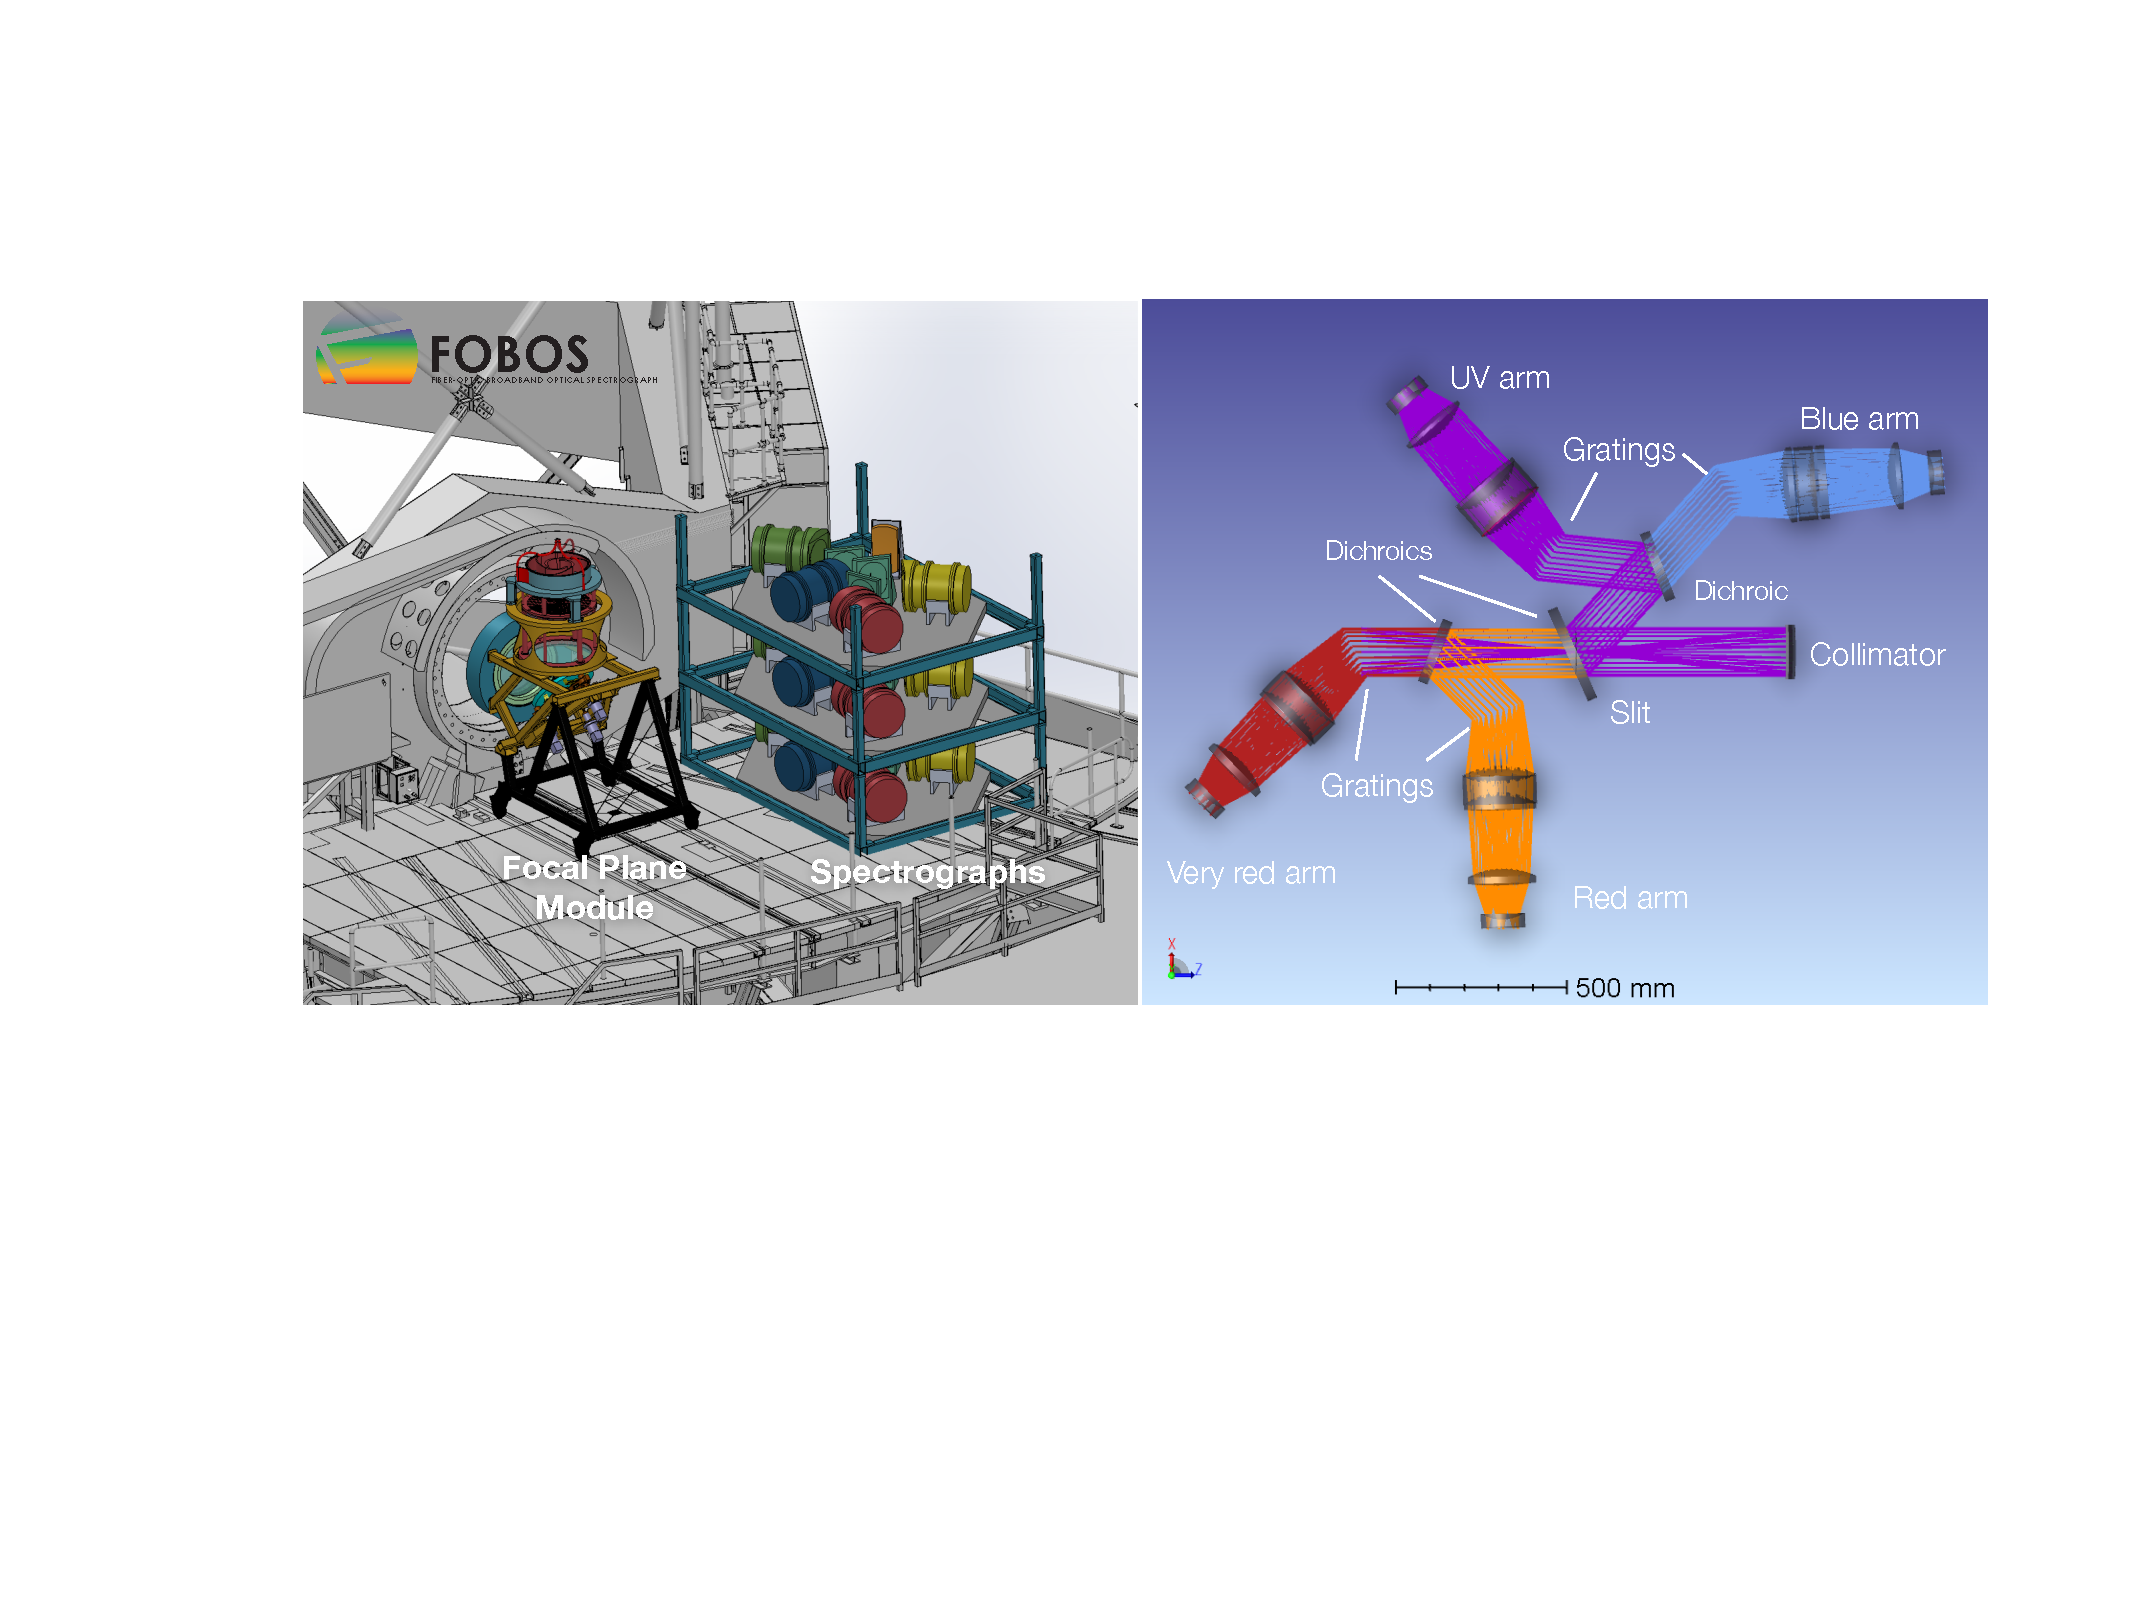
\includegraphics[width=\textwidth]{FOBOS_inst_2019-10-28.pdf}
\caption{\small {\it Left}: Rendering of FOBOS instrument systems
deployed at the Keck II Nasmyth port. {\it Right}: Optical layout of
one of the three four-armed FOBOS spectrographs.}
\label{fig:layout}
\end{figure}

FOBOS inherited much from the conceptual design of a fiber-based
opticl spectrograph for the Thirty-Meter Telescope in a
trade/down-selection study for its Wide-Field Optical Spectrograph
(WFOS); however, it is still in its conceptual design phase. No CDR
package has yet been produced or included in response to this RFI.

% - What are the three primary technical issues or risks?
% - Describe any instrumentation that may require non-US participation. 

The current conceptual designs for all FOBOS sub-systems are briefly
described below. Our risk register assigns the highest risk levels
to:
%
\begin{enumerate}
\item the Starbugs positioning system (the only system provided by a
non-US partner; see Section \ref{sec:starbugs}), specifically
adhesion and control,
\item the micro-assembly fore-optics, specifically their alignment
and manufacturing and assembly process control, and
\item the performance (uniformity and stability) of our calibration
system and calibration procedures.
\end{enumerate}

\begin{wrapfigure}{r}{0.35\textwidth}
\small
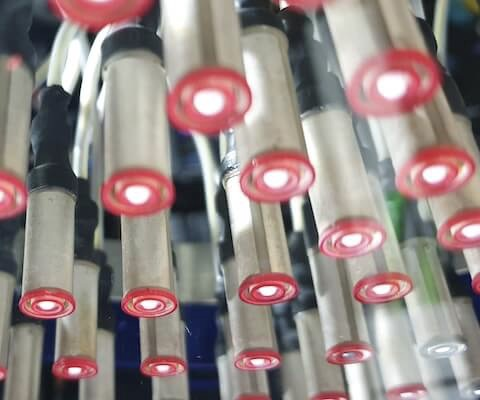
\includegraphics[width=0.35\textwidth]{starbugs_v1.jpg}
\caption{The Starbugs mounted at the focal plane of the AAT. Light
enters from the bottom of the image, where red or gray ``slipper'' of
each Starbug contacts a field plate and is adhered via a leaky
vacuum. The white central area of each Starbug houses the single
fiber apertures. For FOBOS, the contact surface will be the an
optical element of the CLADC, always perpendicular to the gravity
vector, and the Starbugs will be adapted to hold either a single
aperture microlens assembly or an integral-field microlens array
assembly.}
\label{fig:org}
\end{wrapfigure}

\textbf{Focal Plane System.} Light from the Keck II telescope Nasmyth
port (Fig \ref{fig:layout}) passes through the first two 946 mm
diameter lenses of a 3-lens CLADC before encountering a 45$^\circ$
mirror that folds the beam vertically upwards. The horizontal third
lens of the CLADC is positioned at the focal plane above the fold
mirror and serves as the mounting surface for downward-pointing
Starbugs. The risk of Starbug adhesion loss and focal-plane coupling
failure is significantly reduced by using a horizontal mounting
surface (20$^\prime$ diameter). The mounting surface rotates to match
the field rotation of the telescope as it tracks the sky. Each
Starbug patrols zones of up to several arcminutes and can be placed
as close as 10\arcsec. Three back-illuminated fibers embedded in the
housing of each Starbug are combined with a fast, imaging metrology
camera that enables reconfiguration times of as little as 2 minutes.

\noindent \textbf{Focal-Plane Sampling.} Microlens fore-optics
coupled to each fiber demagnify and speed up the telescope beam from
$f/15$ to $f/5$. This provides better coupling of the fiber to the
telescope beam, minimizing losses from focal-ratio degradation, and
provides an $0.8\arcsec$ on-sky diameter of each fiber.
Integral-field observations are accomplished by coupling
large-fill-factor microlens arrays to fiber bundles. Different
Starbug designs accommodate and position one of these payloads in the
focal plane. With stowage zones outside the focal plane, a day-time
procedure switches between different fiber suites: 1) individual
fibers, 600 per spectrograph; 2) A set of 15 multiplexed fiber-bundle
IFUs (per spectrograph), each composed of 37 fibers and spanning up
to 5.6\arcsec; 3) A 30\arcsec-wide monolithic IFU\footnote{This mode
would be unique at Keck. KCWI+KCRM covers 0.36--1.0 $\mu$m and to
achieve $R \sim 3600$ over the full bandpass, KCWI+KCRM reduces its
FoV to 8.4 $\times$ 20.4 arcseconds, an area 5$\times$ smaller than
the FOBOS monolithic IFU.} (1641 fibers). In all cases, $\sim$10\% of
individual fibers are reserved for sky sampling and 5--10
mini-bundles (7 fibers) collect flux calibration standard stars. The
design will accept and take advantage of ground-layer adaptive optics
(GLAO) corrections from an anticipated GLAO system at Keck II. GLAO
improves depth, enables crowded source targeting, and opens new
science territory through spatially-resolved galaxies beyond
$z\sim0.5$.

\textbf{Spectrographs.} Three spectrographs adjacent to the
focal-plane module are fed by a short ($< 10$m) fiber run in order to
preserve UV throughput. Stress-relief features in the cabling reduce
focal-ratio degradation. Each spectrograph uses dichroics to divide
the 140 mm diameter collimated beam into four wavelength channels
with combined, instantaneous coverage from 0.31--1 $\mu$m.
High-efficiency fused-silica etched (FSE) gratings provide
mid-channel spectral resolutions of $R \sim 3500$ for all channels.
The spectrographs use $f/2.25$ refractive cameras, with significant
heritage from the the DESI spectrographs, with 6k$\times$6k, 15
$\mu$m-pixels CCDs; the platescale is such that the images of the
150$\mu$m fiber cores are sampled by 5 pixels. The spectrographs are
mounted in a temperature-controlled housing. The spectrographs will
be held at the expected local nighttime temperature; only the
detectors will be cryogenically cooled using liquid N$_2$. The
estimated end-to-end instrument throughput peaks at 60\% and is
greater than 30\% at all wavelengths.

\noindent \textbf{Calibration System.} FOBOS has a comprehensive
strategy for precise calibrations. Afternoon flat-field and arc-line
exposures will use a carefully illuminated interior dome screen,
acquired specifically for FOBOS calibrations but also a general good
for the Observatory. Nighttime calibrations involve re-orienting the
fold mirror under the focal plane to accept light from a nearby light
source and optical assembly that mimics the telescope pupil.
Afternoon and relative fiber-to-fiber measurements from nighttime
calibrations will be combined to model the instrument$+$sky response
during observations.

\subsection{Technical Maturity}

% - Indicate the technical maturity level of the major elements and the
%   specific instrument maturity of the proposed instrumentation (for each
%   specific Inst #1, Inst#2 etc.), along with the rationale for the
%   assessment (i.e. examples of heritage, existence of breadboards,
%   prototypes, mass/volume and power comparisons to existing units, etc.
%   and any identifications of major long lead items). 

% - Describe the heritage of the instruments and associated sub-systems.
%   Indicate items that are to be developed, as well as any existing
%   hardware or design heritage.
As stated (Section \ref{sec:tech}), the major design elements of
FOBOS are based on proven technologies. Their general technical
maturity and specific risk to the FOBOS design vary:

% - Please fill out the table below regarding each instrument (if
%   applicable). Copy as needed for all instruments. Expand this table as
%   necessary and applicable.

\begin{table}[h!]
\centering
\caption{FOBOS Instrument Table}
\footnotesize
\begin{tabular}{| l | r | r |}
\hline
{\bf Item} & {\bf Value} & {\bf Units} \\
\hline
\hline
Type of instrument      & Spectrograph & \\\hline
Number of spectrographs & 3 & \\\hline
Multiplex & 1800 & single fibers \\
                        & 45 & 37-fiber IFU \\
                        & 1 & 1641-fiber IFU \\\hline
Field of view: Patrol   & 315 & arcmin$^2$ \\\hline
Field of view: Fiber    & 0.5 & arcsec$^2$ \\\hline
Field of view: Mini-IFU & 25 & arcsec$^2$ \\\hline
Field of view: Large-IFU & 705 & arcsec$^2$ \\\hline
Spectral range          & 0.31-1 & $\mu$m \\\hline
Spectral resolution     & 3500 & $R=\lambda/\delta\lambda$ \\\hline
Number of detectors     & 12 & 4 per spectrograph \\\hline
Detector size           & 6k $\times$ 6k & \\\hline
Thermal requirements    & & \\\hline
Size: Spectograph bank  & & m $\times$ m $\times$ m \\\hline
Size: Focal-plane module & & m $\times$ m $\times$ m \\\hline
Data volume (Section \ref{sec:ops})           & $<$100 & Gb \\\hline
Development Schedule    & 100 & months \\\hline
\end{tabular}
\label{tab:instrument}
\end{table}

\section{Facilities}

% - If a site is not yet selected for the project, describe the
%   anticipated approach to conducting site studies, obtaining site
%   permissions, and executing environmental impact studies.
% - Please provide any available site plans. If such plans already address
%   items 2-5 below, these items do not need to be addressed separately.
% - Describe the site and its location, including size, altitude, access,
%   number of buildings, size of building(s) footprint and volume,
%   existing infrastructure, power, internet, environmental considerations
%   and logistics (proximity to major airport, housing and support for
%   construction crews and facility staff etc.).
% - Identify which facilities will be new and which facilities may be
%   pre-existing. Describe any existing facilities and their estimated
%   remaining useful life. Describe any upgrades to existing facilities
%   that will be undertaken. Describe any anticipated shared use of site
%   facilities between the concept being proposed and existing telescopes.
% - For antenna arrays, provide specific infrastructure required such as
%   concrete pad size, communications buildings, etc. for each element in
%   the array. For telescope mirrors, describe infrastructure needed for
%   mirror maintenance, e.g. coating facilities.
% - Describe atmospheric and radio frequency interference (RFI)
%   characteristics of the site insofar as they would affect observations
%   with the concept being proposed.

\section{Operations \& Observation Strategy}
\label{sec:ops}

% - For instrument operations, provide a brief functional description of
%   operational modes, and calibration schemes. This can be documented in
%   the Operations Section. Describe the level of complexity associated
%   with analyzing the data to achieve the scientific objectives of the
%   investigation. Describe the types of data (e.g. bits, images).


% - Please provide operations plans or documents (Concept of Operations). 
% - Provide a description of the facility operations. For example: number
%   of staff required, position types, and 24-hour operation requirements.
% - Provide a description of the science operations. For example:
%   pre-observational planning, data processing/reduction required,
%   coordination with other facilities.
% - Discuss observatory efficiency, e.g. the impact of maintenance and
%   engineering and calibration time on faction of science time
%   availability.
% - Describe scope of engineering activities and time (day or night)
%   needed to maintain calibration and health of telescope/array and
%   instruments.
% - Summarize key software development and any science development
%   required.
% - Summarize any archiving requirements. 
% - Describe any high-level safety policies that will be required for
%   items of particular safety concern.

\noindent \textbf{Data Management System.} FOBOS requires a robust
software suite to handle observational planning, data collection,
processing, and serving. An API (Application Programming Interface)
communicates between the following major sub-systems. {\it The
Doctor}: A database of metadata and performance metrics, as well as
analysis software, to monitor instrument health and predict
performance. {\it The Producer}: Planning, simulation, and execution
of integrated, multiple-pointing observing programs based on {\it
MAISTRO}\footnote{MAISTRO: Modular Artificial Intelligence System for
Target Reallocation and Observing.}, an ``artificial intelligence''
(AI) targeting system that will learn optimization strategies for
user-controlled and multi-program target assignment. {\it The
Accountant}: A data-reduction pipeline with runtime options for both
quick-look and science-ready reductions. {\it The Alchemist}:
Automated derivation of high-level data products (e.g., redshifts).
{\it The Curator}: An archive of all data and data products as well
as a dynamic interface and science platform for visualization and
analysis.

\section{Programmatic Issues \& Schedule}

% - Please provide a programmatic overview that describes the structure of
%   the overall organization including any international partners or
%   university partners etc. and any money or hardware they are providing.
%   Clearly indicate schedule and costs to date highlighting what has
%   already been delivered and/or clearly capturing progress to date, if
%   applicable.
% - Please describe any funding availability challenges and the total
%   impact it had, or may have, to cost and schedule.  Has all required
%   funding been committed?  If not, please explain.  Highlight in-kind
%   contributions in the past and planned from partners.  Clearly describe
%   what the NSF/DOE/Fed Gov funding request is and what it buys.
% - Please describe any unexpected challenges, key risks, and/or current
%   outstanding risks that require(d) significant mitigation which
%   affect/affected cost & schedule.
% - Describe the current top 3 risks to the development of the facility,
%   and proposed mitigation strategies. Please provide a top-level
%   schedule.

\section{Cost}
\label{sec:cost}

% - Provide a high-level facility unique Work Breakdown Structure (WBS)
%   with definitions. 
% - Fill out the cost estimate tables below using the broad bins provided.
%   Note the tables are divided into US Only and with International
%   Partners.  
% - Provide a basis of estimate for project WBS elements at the highest
%   levels (i.e., systems and major subsystems, as indicated in the cost
%   tables below), including internal overhead rates that are applied to
%   costs for labor.  Describe approach or methodology for highest cost
%   element estimates such as analogies, models, expert judgement,
%   construction bids, etc.  Describe cost assumptions made for each
%   element such as any production learning curves, labor and major
%   procurements.  Identify major subcontracted procurements and
%   associated vendors if available.  The “Prior” column is meant to be
%   actual costs incurred. 


%\newpage
%
%\setcounter{page}{1}
%\bibliographystyle{nsf.bst}
%\bibliography{references}

\end{document}


